\chapter{Экспериментальные научные исследования}\label{ch:ch3}

\section{Цели, задачи и план исследования}\label{sec:ch3/sec1}

\textbf{Цели исследования}:
\begin{itemize}
    \item установить прирост в скорости разработки виртуального аппаратного обуспечения;
    \item вычислить падение производительности сгенерированного виртуального аппаратного обеспечения
    относительно аналога написанного на C.
\end{itemize}


\textbf{Задачи}:
\begin{enumerate}[label={\arabic*)}]
    \item реализовать виртуальное устройство классическими методами;
    \item реализовать максимально близкий аналог данного устройства с
        помощью {\mylanguage};
    \item провести замеры времени разработки устройства
        с и без {\mylanguage};
    \item провести замеры времени отклика устройства
        под разными нагрузками;
\end{enumerate}


\section{Реализация устройства}\label{sec:ch3/sec2}

Устройство выполняет задачу сжатия JPEG-картинки.
Данная задача легко поддается измерению, так как:
\begin{itemize}
    \item легко выбрать сложность входных данных -- это
        размер изображения;
    \item возможна векторизация этапов алгоритма;
    \item возможно добавить разные подходы к обработке
        изображения:
        \begin{itemize}
            \item вызов подпрограммы;
            \item отправка данных по сети;
            \item реализация алгоритма устройства.
        \end{itemize}
\end{itemize}

Различные подходы к архитектуре устройства демонстрируют
разные потребности при проектировании эмуляторов аппаратного обеспечения.
Например виртуальное устройство может общаться с реальным, расположенным удаленно,
позволяя получить аппаратное ускорение с замедлением производительности на
скорость сети.

При реализации алгоритма применяется параллелизация внутри этапов кодирования.
Для простоты обозначения, устройство, реализованное на C классическими
методами будет называться C-устройство, а устройство, реализованное с помощью {\mylanguage} --
Python-устройством.
Время сжатия рассчитывается как среднее время сжатия изображения (рис. \ref{fig:image-for-compression})
размером $5000x5000$ пикселей до $10\%$ от объема $1000$ раз.
При весе в $43$ МБ результирующий вес изображения будет равен $4.3$ МБ.


\begin{figure}[!htbp]
    \centering
    \begin{adjustbox}{max totalsize={\textwidth}{\textheight}}
        \includegraphics{images/image_for_compression.jpg}
    \end{adjustbox}
    \caption{Сжимаемое изображение}\label{fig:image-for-compression}
\end{figure}


\begin{figure}[!htbp]
    \centering
    % !TEX encoding = UTF-8 Unicode
% Úτƒ-8 encoded
% http://www.linux.org.ru/forum/general/10357036
\tikzset{
    line/.style={draw, -latex'},
    every join/.style={line},
    u/.style={anchor=south},
    r/.style={anchor=west},
    fxd/.style={text width = 6em},
    it/.style={font={\small\itshape}},
    bf/.style={font={\small\bfseries}},
}
\tikzstyle{base_long} =
    [
        draw,
        on chain,
        on grid,
        align=center,
        minimum height=4ex,
        minimum width = 10ex,
        node distance = 6mm and 60mm,
        text badly centered,
    ]
\tikzstyle{base} =
    [
        draw,
        on chain,
        on grid,
        align=center,
        minimum height=4ex,
        minimum width = 10ex,
        node distance = 6mm and 60mm,
        text badly centered,
        text width=5cm
    ]
\tikzstyle{coord} =
    [
        coordinate,
        on chain,
        on grid
    ]
\tikzstyle{cloud} =
    [
        base,
        ellipse,
        node distance = 3cm,
        minimum height = 2em,
        text width=2cm
    ]
\tikzstyle{decision} =
    [
        base,
        diamond,
        aspect=2,
        node distance = 2cm,
        inner sep = 0pt
    ]
\tikzstyle{block} =
    [
        rectangle,
        base,
        rounded corners,
        minimum height = 2em
    ]
\tikzstyle{print_block} =
    [
        base,
        tape,
        tape bend top=none,
    ]
\tikzstyle{io} =
    [
        base,
        trapezium,
        trapezium left angle = 70,
        trapezium right angle = 110,
    ]
\tikzstyle{prompt} =
    [
        base,
        trapezium,
        trapezium left angle = 90,
        trapezium right angle = 80,
        shape border rotate = 90
    ]
\tikzstyle{disk file} =
    [
        base,
        cylinder,
        aspect=0.2,
    ]
\tikzstyle{process} =
    [
        rectangle,
        base,
    ]
\makeatletter
\pgfkeys{/pgf/.cd,
    subrtshape w/.initial=2mm,
    cycleshape w/.initial=2mm
}
\pgfdeclareshape{parallelshape}{
    \inheritsavedanchors[from=rectangle]
    \inheritanchorborder[from=rectangle]
    \inheritanchor[from=rectangle]{north}
    \inheritanchor[from=rectangle]{center}
    \inheritanchor[from=rectangle]{west}
    \inheritanchor[from=rectangle]{east}
    \inheritanchor[from=rectangle]{mid}
    \inheritanchor[from=rectangle]{base}
    \inheritanchor[from=rectangle]{south}
    \backgroundpath{
        \southwest \pgf@xa=\pgf@x \pgf@ya=\pgf@y
        \northeast \pgf@xb=\pgf@x \pgf@yb=\pgf@y
        \def\ppd@offset{\pgfpoint{\pgfutil@tempdima}{0ex}}
        \def\ppd@offsetm{\pgfpoint{-\pgfutil@tempdima}{0ex}}
        \pgfpathmoveto{\pgfqpoint{\pgf@xa}{\pgf@ya}}
            \pgfpathlineto{\pgfqpoint{\pgf@xb}{\pgf@ya}}
        \pgfpathclose
        \pgfpathmoveto{\pgfqpoint{\pgf@xb}{\pgf@yb}}
            \pgfpathlineto{\pgfqpoint{\pgf@xa}{\pgf@yb}}
        \pgfpathclose
    }
}
\pgfdeclareshape{subrtshape}{
    \inheritsavedanchors[from=rectangle]
    \inheritanchorborder[from=rectangle]
    \inheritanchor[from=rectangle]{north}
    \inheritanchor[from=rectangle]{center}
    \inheritanchor[from=rectangle]{west}
    \inheritanchor[from=rectangle]{east}
    \inheritanchor[from=rectangle]{mid}
    \inheritanchor[from=rectangle]{base}
    \inheritanchor[from=rectangle]{south}
    \backgroundpath{
        \southwest \pgf@xa=\pgf@x \pgf@ya=\pgf@y
        \northeast \pgf@xb=\pgf@x \pgf@yb=\pgf@y
        \pgfmathsetlength\pgfutil@tempdima{\pgfkeysvalueof{/pgf/subrtshape w}}
        \def\ppd@offset{\pgfpoint{\pgfutil@tempdima}{0ex}}
        \def\ppd@offsetm{\pgfpoint{-\pgfutil@tempdima}{0ex}}
        \pgfpathmoveto{\pgfqpoint{\pgf@xa}{\pgf@ya}}
        \pgfpathlineto{\pgfqpoint{\pgf@xb}{\pgf@ya}}
        \pgfpathlineto{\pgfqpoint{\pgf@xb}{\pgf@yb}}
        \pgfpathlineto{\pgfqpoint{\pgf@xa}{\pgf@yb}}
        \pgfpathclose
        \pgfpathmoveto{\pgfpointadd{\pgfpoint{\pgf@xa}{\pgf@yb}}{\ppd@offsetm}}
        \pgfpathlineto{\pgfpointadd{\pgfpoint{\pgf@xa}{\pgf@ya}}{\ppd@offsetm}}
        \pgfpathlineto{\pgfpointadd{\pgfpoint{\pgf@xb}{\pgf@ya}}{\ppd@offset}}
        \pgfpathlineto{\pgfpointadd{\pgfpoint{\pgf@xb}{\pgf@yb}}{\ppd@offset}}
        \pgfpathclose
    }
}
\pgfdeclareshape{cyclebegshape}{
    \inheritsavedanchors[from=rectangle]
    \inheritanchorborder[from=rectangle]
    \inheritanchor[from=rectangle]{north}
    \inheritanchor[from=rectangle]{center}
    \inheritanchor[from=rectangle]{west}
    \inheritanchor[from=rectangle]{east}
    \inheritanchor[from=rectangle]{mid}
    \inheritanchor[from=rectangle]{base}
    \inheritanchor[from=rectangle]{south}
    \backgroundpath{
        \southwest \pgf@xa=\pgf@x \pgf@ya=\pgf@y
        \northeast \pgf@xb=\pgf@x \pgf@yb=\pgf@y
        \pgfmathsetlength\pgfutil@tempdima{\pgfkeysvalueof{/pgf/cycleshape w}}
        \pgfpathmoveto{\pgfqpoint{\pgf@xa}{\pgf@ya}}
\pgfpathlineto{\pgfpointadd{\pgfpoint{\pgf@xa}{\pgf@yb}}{\pgfpoint{0ex}{-\pgfutil@tempdima}}}
\pgfpathlineto{\pgfpointadd{\pgfpoint{\pgf@xa}{\pgf@yb}}{\pgfpoint{\pgfutil@tempdima}{0ex}}}
\pgfpathlineto{\pgfpointadd{\pgfpoint{\pgf@xb}{\pgf@yb}}{\pgfpoint{-\pgfutil@tempdima}{0ex}}}
\pgfpathlineto{\pgfpointadd{\pgfpoint{\pgf@xb}{\pgf@yb}}{\pgfpoint{0ex}{-\pgfutil@tempdima}}}
\pgfpathlineto{\pgfqpoint{\pgf@xb}{\pgf@ya}}
        \pgfpathclose
    }
}
\pgfdeclareshape{cycleendshape}{
    \inheritsavedanchors[from=rectangle]
    \inheritanchorborder[from=rectangle]
    \inheritanchor[from=rectangle]{north}
    \inheritanchor[from=rectangle]{center}
    \inheritanchor[from=rectangle]{west}
    \inheritanchor[from=rectangle]{east}
    \inheritanchor[from=rectangle]{mid}
    \inheritanchor[from=rectangle]{base}
    \inheritanchor[from=rectangle]{south}
    \backgroundpath{
        \southwest \pgf@xa=\pgf@x \pgf@ya=\pgf@y
        \northeast \pgf@xb=\pgf@x \pgf@yb=\pgf@y
        \pgfmathsetlength\pgfutil@tempdima{\pgfkeysvalueof{/pgf/cycleshape w}}
        \pgfpathmoveto{\pgfqpoint{\pgf@xb}{\pgf@yb}}
\pgfpathlineto{\pgfpointadd{\pgfpoint{\pgf@xb}{\pgf@ya}}{\pgfpoint{0ex}{\pgfutil@tempdima}}}
\pgfpathlineto{\pgfpointadd{\pgfpoint{\pgf@xb}{\pgf@ya}}{\pgfpoint{-\pgfutil@tempdima}{0ex}}}
\pgfpathlineto{\pgfpointadd{\pgfpoint{\pgf@xa}{\pgf@ya}}{\pgfpoint{\pgfutil@tempdima}{0ex}}}
\pgfpathlineto{\pgfpointadd{\pgfpoint{\pgf@xa}{\pgf@ya}}{\pgfpoint{0ex}{\pgfutil@tempdima}}}
\pgfpathlineto{\pgfqpoint{\pgf@xa}{\pgf@yb}}
        \pgfpathclose
    }
}
\makeatother
\tikzstyle{subroutine} =
    [
        base,
        subrtshape,
    ]
\tikzstyle{cyclebegin} =
    [
        base,
        cyclebegshape,
    ]
\tikzstyle{cycleend} =
    [
        base,
        cycleendshape,
    ]
\tikzstyle{connector} =
    [
        base,
        circle,
    ]

\tikzstyle{parallel} =
    [
        base_long,
        parallelshape,
    ]
\begin{tikzpicture}[%
    start chain=going below,    % General flow is top-to-bottom
    node distance=6mm and 30mm, % Global setup of box spacing
    ]
        \node [cloud] (start) {\small Начало};
        \node [cyclebegin] (foreach commit start) [below = 2cm of start] {\small Для каждого коммита в системе контроля версий};

        \node [decision] (if small diff) [below = 4cm of foreach commit start] {\small Разница с предыдущим коммитом меньше 2х часов?};

        \node [block] (small diff) [below left = 7cm of if small diff] {\small Коммиты принадлежат к непрерывной сессии программирования};
        \node [block] (session time)
                      [below = 3.5cm of small diff]
                      {\small Затраченное время равно разницы между первым и последним коммитом в сессии};

        \node [block] (not small diff) [below right = 7.1cm of if small diff] {\small Коммиты принадлежат к разным сессиям программирования};

        \node [cycleend] (foreach commit end) [below = 16cm of foreach commit start] {\small Для каждого коммита в системе контроля версий};
        \node [block] (sum) [below = 2.5cm of foreach commit end] {\small Сложение времени всех сессий};
        \node [cloud] (end) [below = 2.5cm of sum] {\small Конец};

        \draw [->] (start) -- (foreach commit start);
        \draw [->] (foreach commit start) -- (if small diff);
        \draw [->] (if small diff.west) -- (-4.95, -6) node [midway, above, sloped] (yes) {Да} -- (small diff.north);
        \draw [->] (if small diff.east) -- (5, -6) node [midway, above, sloped] (no) {Нет} -- (not small diff);
        \draw [->] (small diff) -- (session time);
        \draw [->] (session time.south) -- (-4.95, -16.5) -- (0, -16.5) -- (foreach commit end.north);
        \draw [->] (not small diff.south) -- (5, -16.5) -- (0, -16.5) -- (foreach commit end.north);
        \draw [->] (foreach commit end) -- (sum);
        \draw [->] (sum) -- (end);



\end{tikzpicture}

    \caption{Алгоритм подсчета времени, затраченного на разработку устройства.}\label{fig:git-hours}
\end{figure}

\subsection{Устройство со встроенной логикой}\label{sec:ch3/sec2/sec1}

Данное устройство реализует алгоритм сжатия JPEG картинки в себе.

\subsubsection{Особенности реализации}\label{sec:ch3/sec2/sec1/sec1}

Многопоточность в Python, в отличие от C не дает прироста производительности,
поэтому для параллелизации задач пишутся либо C-модули для языка, либо используются
многопроцессные вычисления, когда запускается $N$ интерпретаторов питона, общающихся
между собой через разделяемую память. Это накладывает определенные издержки на запуск
и сериализацию/десериализацию сообщений, чего нет в C-коде с применением OpenMP или
грамотной расстановкой мьютексов.

\begin{longtable}{| p{3cm} | p{3cm} | p{3cm} | p{3cm} | p{3cm} |}
    \hline
        \multirow{2}{*}{Метрика} &
        \multicolumn{2}{c|}{Разработка с нуля} &
        \multicolumn{2}{c|}{Использование библиотеки} \\
    \cline{2-5} &
        C устройство &
        Python устройство &
        C устройство &
        Python устройство \\
    \hline
        Время разработки в человеко-часах &
        $100$ &
        $50$ &
        $35$ &
        $10$ \\
    \hline
        Время сжатия (сек.)&
        $3.915$  (рис. \ref{fig:hist-handmade-c-dev}) &
        $18.548$ (рис. \ref{fig:hist-handmade-py-dev}) &
        $1.871$  (рис. \ref{fig:hist-lib-c-dev}) &
        $2.786$  (рис. \ref{fig:hist-lib-py-dev}) \\
    \hline
\end{longtable}

\begin{figure}[!htbp]
    \centering
    \begin{adjustbox}{max totalsize={\textwidth}{\textheight}}
        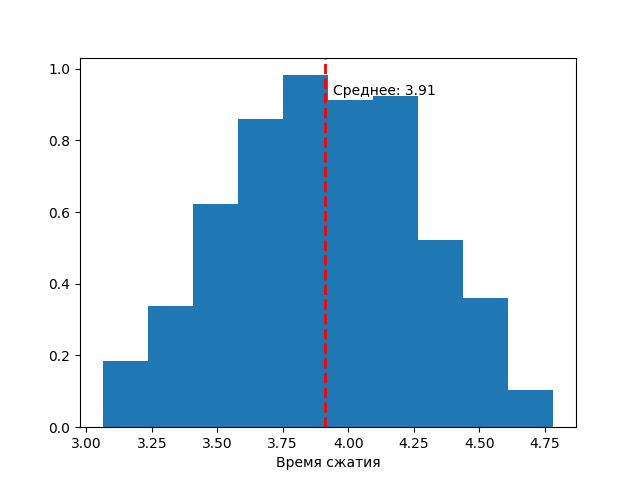
\includegraphics{images/hist-handmade-c-dev.png}
    \end{adjustbox}
    \caption{Время сжатия разработанным с нуля C-устройством.}\label{fig:hist-handmade-c-dev}
\end{figure}


\begin{figure}[!htbp]
    \centering
    \begin{adjustbox}{max totalsize={\textwidth}{\textheight}}
        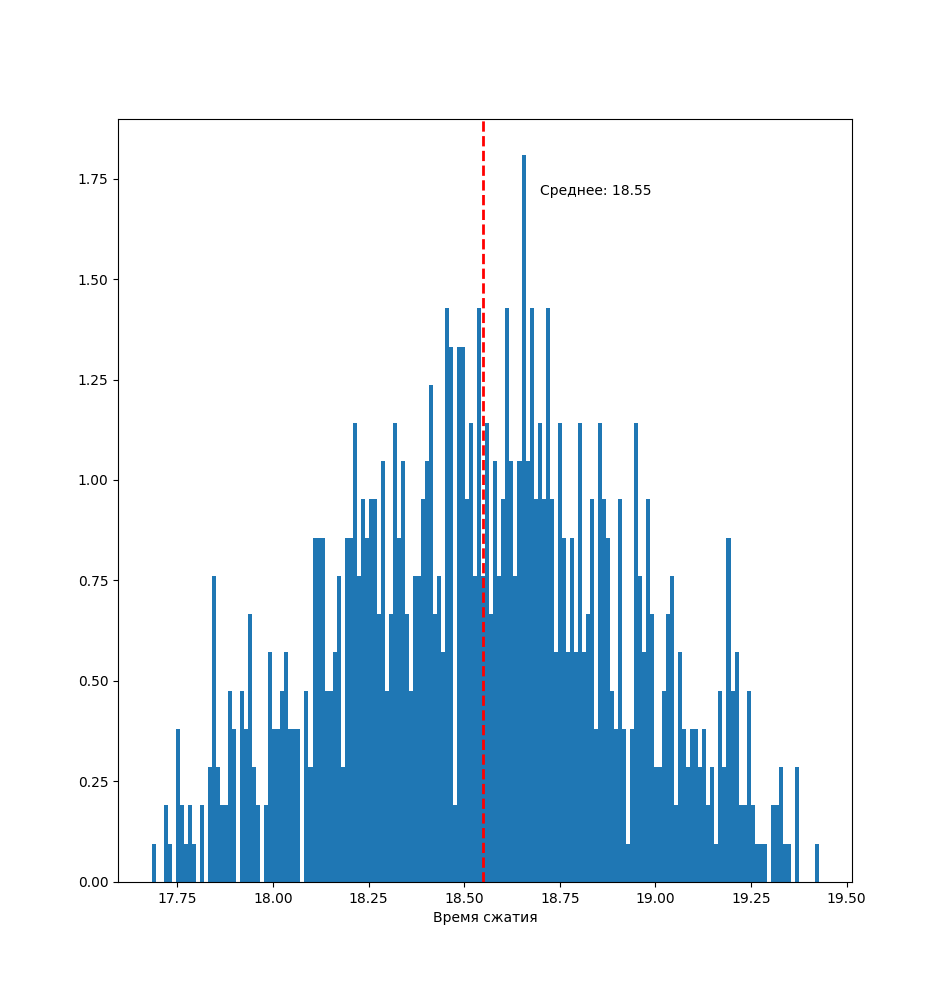
\includegraphics{images/hist-handmade-py-dev.png}
    \end{adjustbox}
    \caption{Время сжатия разработанным с нуля Python-устройством.}\label{fig:hist-handmade-py-dev}
\end{figure}


\begin{figure}[!htbp]
    \centering
    \begin{adjustbox}{max totalsize={\textwidth}{\textheight}}
        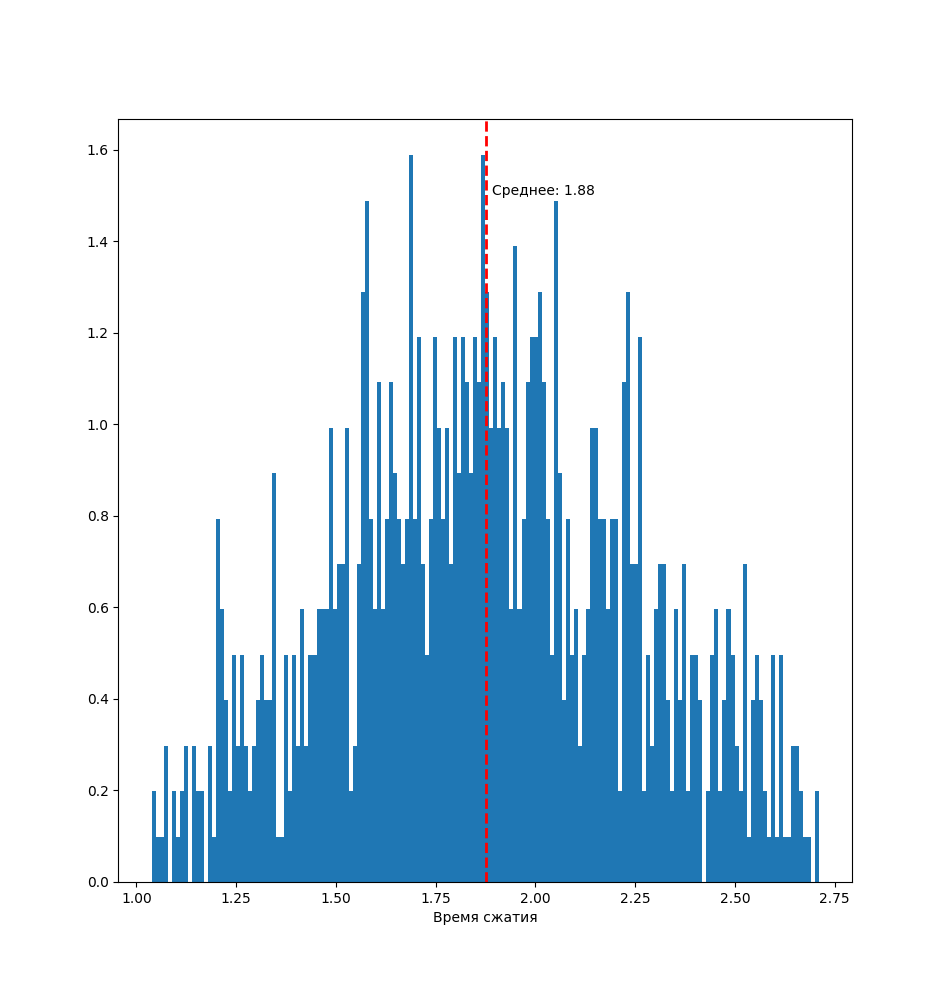
\includegraphics{images/hist-lib-c-dev.png}
    \end{adjustbox}
    \caption{Время сжатия C-устройством, использующим библиотеку.}\label{fig:hist-lib-c-dev}
\end{figure}


\begin{figure}[!htbp]
    \centering
    \begin{adjustbox}{max totalsize={\textwidth}{\textheight}}
        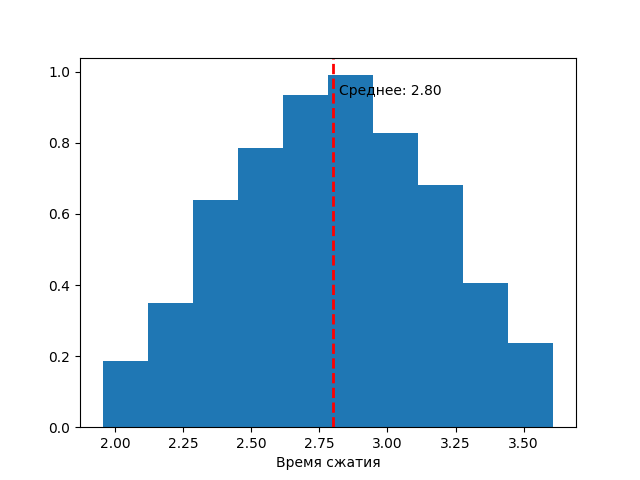
\includegraphics{images/hist-lib-py-dev.png}
    \end{adjustbox}
    \caption{Время сжатия Python-устройством, использующим библиотеку.}\label{fig:hist-lib-py-dev}
\end{figure}

\textbf{Вывод:} при создании устройства на C, очевидна разница
в скорости разработки -- имплементация устройства с нуля
требует серьезных усилий и знаий от программиста, большое количество
времени, как и возможные деструктивные ошибки связаны с управлением
памятью. Создание устройства с помощью {\mylanguage} позволяет
сократить время разработки вдвое, так как основной фокус програмиста
занят не второстепенными вещами, а реализацией алгоритма.
В то же время, использование библиотеки радикально сокращает
время разработки, но, в случае C-устройства, большое количество
времени все еще отнимает управление памятью.
Производительность, при реализации устройств без сторонних
библиотек, показывает, что Python-устройство в $4.7$ раза
медленнее аналогичного C-устройства. При использовании
библиотек, разрыв сокращается до $1.5$ раза, что связано
с накладными расходами -- библиотека обработки изображений
для Python написана как модуль, на языке C, что обеспечивает
максимальную производительность самого вычислительноемкого этапа.

\subsection{Устройство с удаленной логикой}\label{sec:ch3/sec2/sec2}

Данное устройство не реализует алгоритм сжатия JPEG картинки в себе,
а отправляет изображение внешнему обработчику,
возвращая полученное сжатое изображение в гостевую ОС.
Данная архитектура позволяет иметь, например, оптимизированный
кластер для обработки информации, к которому подключаются и с
которым общаются виртуальные устройства.

\subsubsection{Устройство, работающее через сеть}\label{sec:ch3/sec2/sec2/sec1}

В данном случае обработчиком выступает обрабатывающий узел в сети.
Реализация собственного сетевого взаимодействия не проводилась
и для него использовались сторонние библиотеки.
Данное устройство -- расширение разработанного в \ref{sec:ch3/sec2/sec1/sec1}.

\begin{longtable}{| p{5cm} | p{5cm} | p{5cm} |}
    \hline
        Метрика &
        C устройство &
        Python устройство \\
    \hline
        Суммарное Время разработки в человеко-часах &
        $45$ ($+10$) &
        $14$ ($+4$) \\
    \hline
        Время сжатия (сек.)&
        $2.341$ ($+0.47$) (рис. \ref{fig:hist-lib-c-network}) &
        $3.533$ ($+0.75$) (рис. \ref{fig:hist-lib-py-network}) \\
    \hline
\end{longtable}


\begin{figure}[!htbp]
    \centering
    \begin{adjustbox}{max totalsize={\textwidth}{\textheight}}
        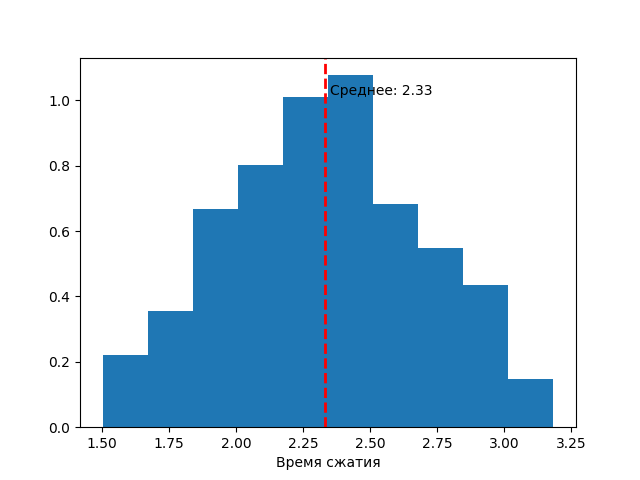
\includegraphics{images/hist-lib-c-network.png}
    \end{adjustbox}
    \caption{Время сжатия C-устройством по сети.}\label{fig:hist-lib-c-network}
\end{figure}


\begin{figure}[!htbp]
    \centering
    \begin{adjustbox}{max totalsize={\textwidth}{\textheight}}
        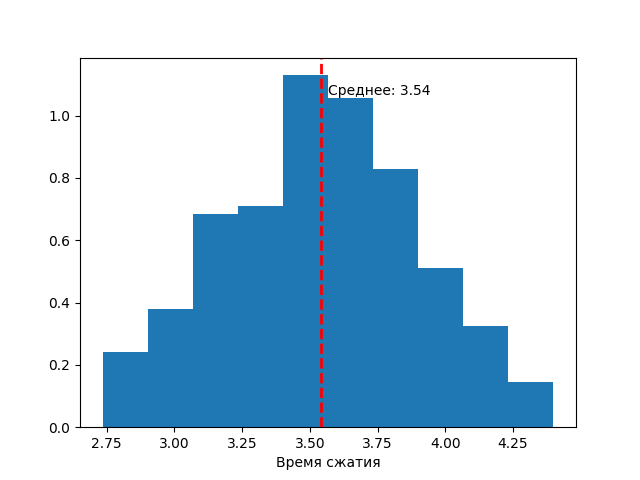
\includegraphics{images/hist-lib-py-network.png}
    \end{adjustbox}
    \caption{Время сжатия Python-устройством по сети.}\label{fig:hist-lib-py-network}
\end{figure}

\textbf{Вывод:} данный эксперимент показывает, что добавление новых возможностей,
уже реализованных сторонними библиотеками, для C-устройства занимает больше времени,
чем для Python-устройства при сопоставимой производительности.

\subsubsection{Устройство, работающее с подпроцессом}\label{sec:ch3/sec2/sec2/sec2}

В данном случае обработчиком выступает запускаемый подпроцесс сжатия
изображения. В качестве подпроцесса использовалась существующая программа
для сжатия JPEG-изображений -- \texttt{jpegoptim} \cite{jpegoptim}.
Данный подход позволяет быстро реализовать сложную логику в ситуации, когда
для нее не существует библиотеки.

\begin{longtable}{| p{5cm} | p{5cm} | p{5cm} |}
    \hline
    Метрика & C-устройство & Python-устройство \\
    \hline
        Время разработки в человеко-часах &
        $25$ ($-30$) &
        $10$ ($-2$) \\
    \hline
        Быстродействие &
        $2.031$ ($+0.16$) (рис. \ref{fig:hist-exec-c-dev}) &
        $3.246$ ($+0.46$) (рис. \ref{fig:hist-exec-py-dev}) \\
    \hline
\end{longtable}

\begin{figure}[!htbp]
    \centering
    \begin{adjustbox}{max totalsize={\textwidth}{\textheight}}
        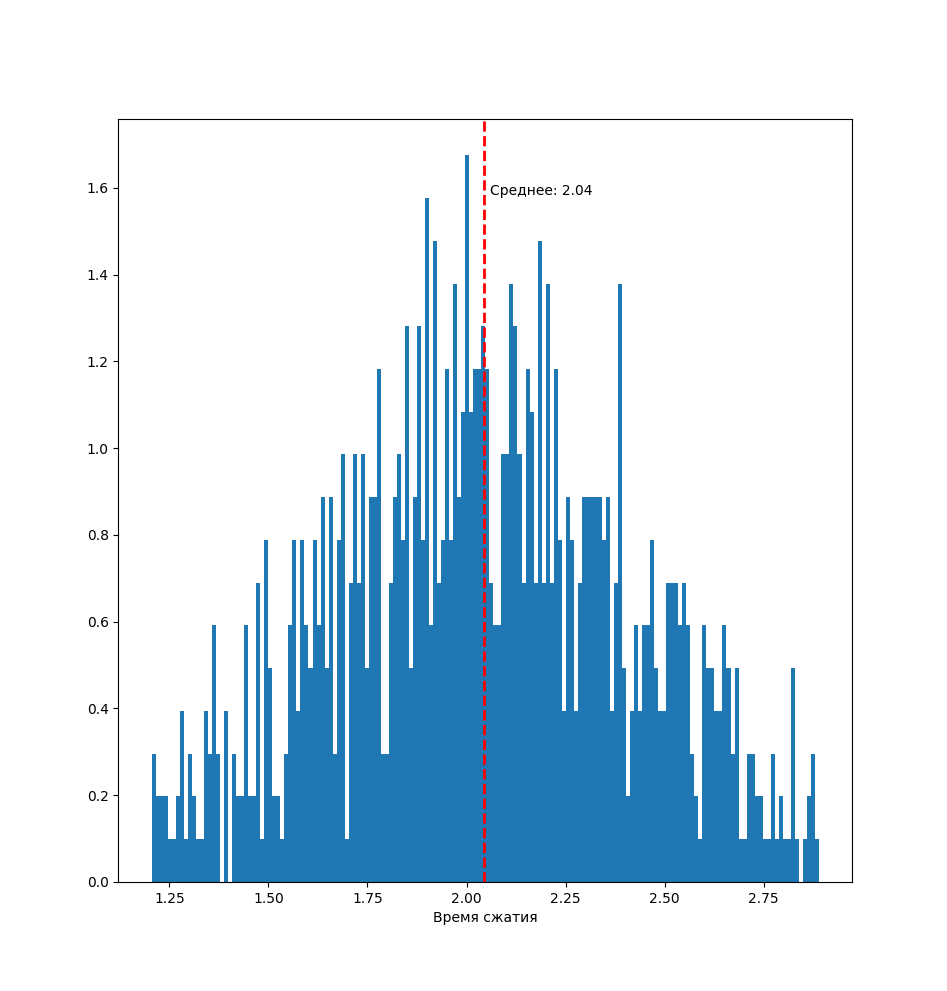
\includegraphics{images/hist-exec-c-dev.png}
    \end{adjustbox}
    \caption{Время сжатия C-устройством через подпроцесс.}\label{fig:hist-exec-c-dev}
\end{figure}


\begin{figure}[!htbp]
    \centering
    \begin{adjustbox}{max totalsize={\textwidth}{\textheight}}
        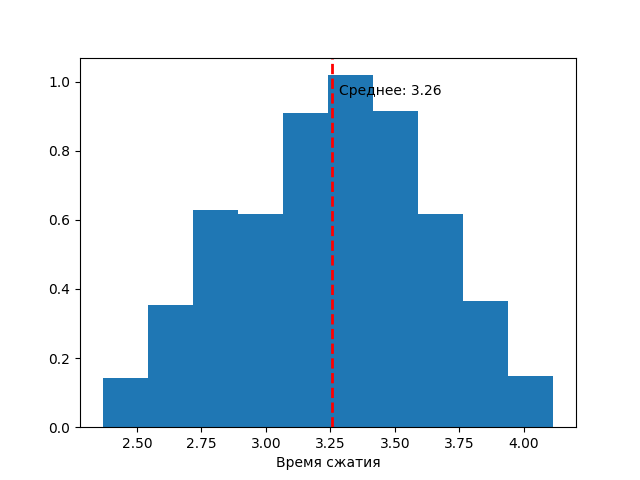
\includegraphics{images/hist-exec-py-dev.png}
    \end{adjustbox}
    \caption{Время сжатия Python-устройством через подпроцесс.}\label{fig:hist-exec-py-dev}
\end{figure}

\textbf{Вывод:} данный эксперимент является достаточно специфичным, так как отражает процесс
решения узкого класса задач. В то же время, решение является лучшим по соотношению
времени разработки к быстродействию устройства.
Это вызвано тем, что использовалось существующее ПО и временные затраты на
организацию управления памятью в C-устройстве незначительны.
В то же время, быстродействие данного устройства лишь немногим лучше устройства,
реализованного в \ref{sec:ch3/sec2/sec2/sec1}. Это является следствием издержек
системных вызовов для запуска подпроцессов обработки изображения.


\textbf{Итог:} в данной главе рассмотрены различные варианты реализации виртуального
устройства, проведено сравнение классического метода реализации виртуального устройства
QEMU и реализация виртуального устройства с помощью {\mylanguage}.
Во всех экспериментах устройство, реализованное через {\mylanguage} выделяется
скоростью разработки при небольшом падении в производительности.
